\documentclass[12pt,a4paper,oneside]{article}

\usepackage[italian]{babel}
\usepackage[T1]{fontenc}
\usepackage[utf8]{inputenc}
\usepackage[margin=1in]{geometry}
\usepackage{graphicx}

\begin{document}
	
	\title{N-bodies simulation\\Assignment programmazione concorrente e distribuita}
	\author{Filippo Barbari}
	\date{}%no date
	\maketitle
	
	\tableofcontents
	\newpage
	
	\section{Analisi}
	\subsection{Descrizione della simulazione}
	Questa simulazione è una variante della nota "simulazione di $N$ corpi". La simulazione è composta da:
	\begin{itemize}
		\item un numero $N$ di corpi ciascuno dotato di massa ma incorporeo (non ha una dimensione)
		\item un dominio bidimensionale finito di forma rettangolare e allineato con gli assi cartesiani
		\item una forza repulsiva tra i corpi (descritta in dettaglio di seguito)
		\item una forza d'attrito applicata sui singoli corpi
	\end{itemize}
	
	\subsection{Analisi dell'algoritmo}
	\subsection{Analisi delle dipendenze tra dati}
	
	\section{Design}
	\subsection{Using two barriers}
	
	\section{Dettagli implementativi}
	
	\section{Valutazione prestazioni}
	\subsection{Tempi di esecuzione}
	I tempi riportati di seguito fanno riferimento ad un'esecuzione parallela che utilizza 8 thread.
	
	\hfill
	\begin{minipage}{.4\textwidth}
		Senza GUI
		
		\begin{tabular}{|l|l|l|}
			\hline
			\multicolumn{1}{|c|}{\textbf{N. corpi}} & \multicolumn{1}{c|}{\textbf{N. step}} & \multicolumn{1}{c|}{\textbf{Tempo}} \\ \hline
			100 & 1000 & 0,11 \\ \hline
			100 & 10000 & 0,602 \\ \hline
			100 & 50000 & 2,939 \\ \hline
			1000 & 1000 & 1,403 \\ \hline
			1000 & 10000 & 14,139 \\ \hline
			1000 & 50000 & 65,73 \\ \hline
			5000 & 1000 & 47,193 \\ \hline
			5000 & 10000 & 474,334 \\ \hline
			5000 & 50000 & 2351,408 \\ \hline
		\end{tabular}
	\end{minipage}
	\hfill
	\begin{minipage}{.4\textwidth}
		Con GUI
		
		\begin{tabular}{|l|l|l|}
			\hline
			\multicolumn{1}{|c|}{\textbf{N. corpi}} & \multicolumn{1}{c|}{\textbf{N. step}} & \multicolumn{1}{c|}{\textbf{Tempo}} \\ \hline
			100 & 1000 & 0,117 \\ \hline
			100 & 10000 & 0,74 \\ \hline
			100 & 50000 & 3,364 \\ \hline
			1000 & 1000 & 3,101 \\ \hline
			1000 & 10000 & 30,25 \\ \hline
			1000 & 50000 & 143,894 \\ \hline
			5000 & 1000 & 68,841 \\ \hline
			5000 & 10000 & 673,219 \\ \hline
			5000 & 50000 & 3328,55 \\ \hline
		\end{tabular}
	\end{minipage}
	\hfill

	\subsection{Speedup}
	Valori speedup (misurati con 1000 corpi e 10000 step).
	
	\begin{figure}[!ht]
		\centering
		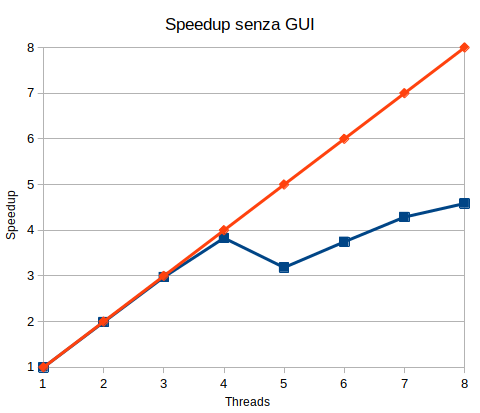
\includegraphics[width=0.7\linewidth]{speedup-no-gui}
		\caption{}
		\label{fig:speedup-no-gui}
	\end{figure}
	
	\begin{figure}[!ht]
		\centering
		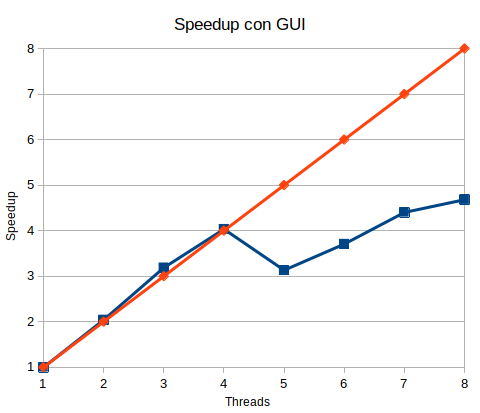
\includegraphics[width=0.7\linewidth]{speedup-gui}
		\caption{}
		\label{fig:speedup-gui}
	\end{figure}
	

	\hfill
	\begin{minipage}{.4\textwidth}
		Senza GUI

		\begin{tabular}{|c|c|}
			\hline
			\textbf{Threads} & \textbf{Time} \\ \hline
			1 & 84,689 \\ \hline
			2 & 42,575 \\ \hline
			3 & 28,473 \\ \hline
			4 & 22,11 \\ \hline
			5 & 26,59 \\ \hline
			6 & 22,603 \\ \hline
			7 & 19,744 \\ \hline
			8 & 18,464 \\ \hline
		\end{tabular}
	\end{minipage}
	\hfill
	\begin{minipage}{.4\textwidth}
		Con GUI

		\begin{tabular}{|c|c|}
			\hline
			\textbf{Threads} & \textbf{Time} \\ \hline
			1 & 86,474 \\ \hline
			2 & 42,393 \\ \hline
			3 & 27,135 \\ \hline
			4 & 21,44 \\ \hline
			5 & 27,606 \\ \hline
			6 & 23,332 \\ \hline
			7 & 19,645 \\ \hline
			8 & 18,473 \\ \hline
		\end{tabular}
	\end{minipage}
	
	\subsection{Strong scaling efficiency}
	\begin{figure}[!ht]
		\centering
		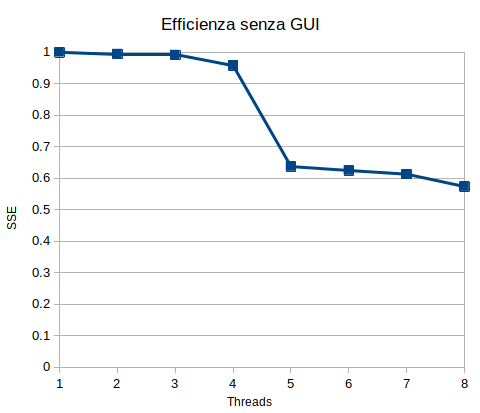
\includegraphics[width=0.7\linewidth]{sse-no-gui}
		\caption{}
		\label{fig:sse-no-gui}
	\end{figure}
	
	\begin{figure}[!ht]
		\centering
		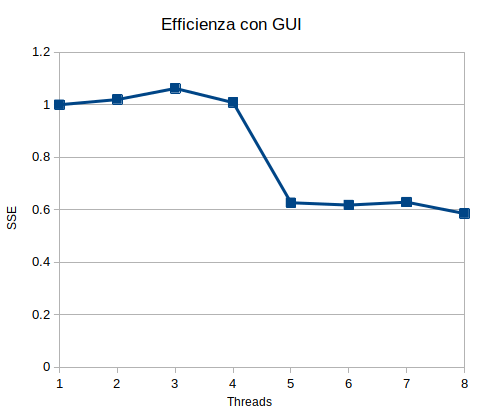
\includegraphics[width=0.7\linewidth]{sse-gui}
		\caption{}
		\label{fig:sse-gui}
	\end{figure}
	
	\subsection{Profiling}
	Numero di thread?
	Utilizzo memoria?
	\subsection{Throughput}
\end{document}